%
% Chapter 2
%
\chapter{Background}\label{chap:background}
\paragraph{}

Nowadays, the authenticity and accessibility of academic certificates play a crucial role in ensuring trust and credibility in various
domains, ranging from education to employment and beyond.
The current and traditional \textit{paper-based} system of issuing and verifying academic certificates is not only time consuming but also prone to a lot of fraud and manipulation.
The widespread issue of counterfeit certificates\cite{certCounterfeitAdv, certCounterfeitRid, Rodrigues_2023}, coupled with inefficient verification processes and the risk of loss or damage, highlight the need for a more reliable and secure academic certificate registry system.

The current system of academic certificate registry faces numerous challenges. Firstly, the reliance on paper-based is problematic. Paper-based certificates are easily forged and tampered with. This undermines the credibility and integrity of academic qualifications. Secondly, the manual verification process is
time-consuming and prone to errors, leading to delays in credential validation, possible fraudulent activities and also potential loss of revenue for institutions due to
errors in the manual release. Thirdly, since the issue of certificates from educational institutions are mostly centralized, this intensify the difficulty
of maintaining a unified and updated registry.

\section{Overview}\label{sec:overview}
\paragraph{}

There are several approaches to address the challenges of the traditional academic certificate registry system. One such solution is the implementation of centralized databases managed by government or regulatory authorities,
where educational institutions are required to submit digital copies of certificates for verification purposes~\cite{LinWays}.
Other solution is the adoption of distributed storage systems where data is stored across multiple nodes in a network, but not all nodes have the same equal authority and the data is not fully decentralized. Which means that there's an entity that has control over the network~\cite{sharples2016blockchain}.
This solution is not centralized neither fully distributed but have a mix of both approaches that makes the system more secure and reliable than only a centralized one.
The third solution that we will approach is a fully distributed one that offers a decentralized, secure, and tamper-proof ledger. In this system, certificates can be stored and verified without a single entity having control over the network. Instead, the control is distributed across multiple nodes, making the system more resilient to tampering and centralized failures. Each transaction is validated by a consensus mechanism, ensuring that only legitimate entries are added to the ledger. This decentralized nature means that no single entity can unilaterally alter or manipulate the stored certificates, enhancing security and trustworthiness. This solution is based on the \textit{blockchain technology}~\cite{app14020706, saleh2020blockchain}.

\section{Centralized Storage Systems}\label{sec:centralized-systems}
\paragraph{}

Several attempts have been made to address the challenges of the traditional academic certificate registry system.
As we can see in the Figure~\ref{fig:centralized-system}, one such solution is the implementation of \textit{centralized databases}~\cite{OLSON200971} managed by government or regulatory authorities, where educational institutions are required to
submit digital copies of certificates for verification purposes. Although this approach aims to centralize certificate records and simplify the verification process, it still faces challenges
such as the risk and concerns of data privacy and security, interoperability issues between different databases and the need of a trusted third party to manage the database.
This storage systems often only store grades and not the actual certificates which undermines the credibility and integrity of academic qualifications.
Moreover, the reliance on a central authority to manage the certificate increases the risk of fraud and manipulation, as the data can be altered or deleted by a single entity.

\begin{figure}[h]\label{fig:centralized-system}
    \begin{center}
        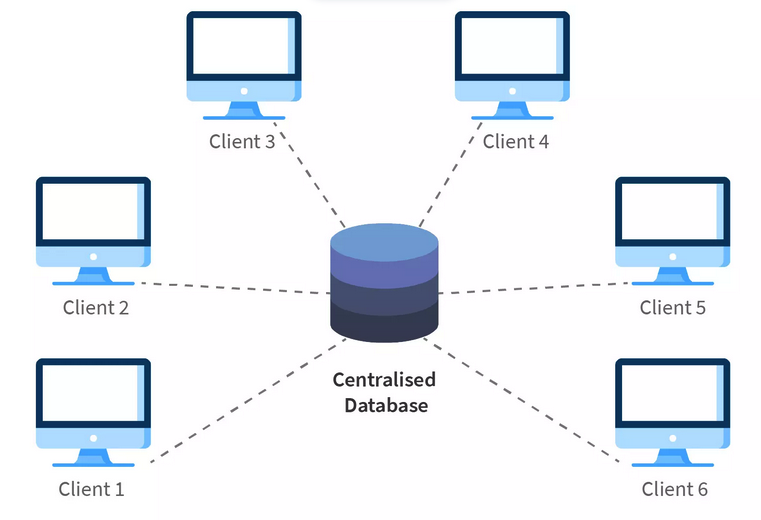
\includegraphics[width=0.8\textwidth]{assets/centralized-database.png}
        \caption{Centralized System~\cite{centralizedDB}.}
    \end{center}
\end{figure}

\section{Distributed Storage Systems}\label{sec:distributed-systems}
\paragraph{}

Another solution to address the challenges of the traditional academic certificate registry system could be the adoption of distributed storage systems where the data is stored in multiple nodes in a network.
Has we see in the Figure~\ref{fig:distributed-system}, different that what we've seen in the previous section, the data is replicated across multiple nodes of the system, ensuring that the data is available even if some nodes fail. However, not all nodes have the same equal authority which means that
it is not fully decentralized.

\vspace{.25cm}
\begin{figure}[h]\label{fig:distributed-system}
    \begin{center}
        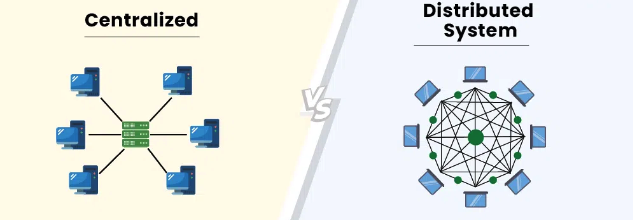
\includegraphics[width=0.8\textwidth]{assets/centralized-vs-distributed.png}
        \caption{Centralized vs Distributed Systems~\cite{centralizedVsDistributed}.}
    \end{center}
\end{figure}

In the context of education, distributed storage systems can significantly enhance the reliability and security of academic certificate validation.
Educational institutions, accrediting bodies, and employers can benefit from a system where academic records are distributed across a network of trusted nodes,
rather than being stored in a single central repository.
The key benefits of this approach in the education sector include improved security, enhanced reliability and scalability.

\section{Blockchain}\label{sec:blockchain}
\paragraph{}

Recently, another solution that have being proposed is the adoption of blockchain technology for academic certificate registry. As we can see in Figure \ref{fig:blockchain-vs-database}, also being a distributed storage system, this technology goes beyond by offering a fully decentralized solution.
Blockchain offers a decentralized, secure and tamper-proof ledger where certificates can be stored and verified.
\textit{Tamper-proof ledger} is a system designed to maintain records where once information is added, it cannot be altered or deleted. This is achieved through a combination of cryptographic techniques and a distributed network of computers (nodes) that each hold a copy of the ledger.
Every transaction or entry is verified by these nodes, and any attempt to change past records would require altering the data on a majority of these nodes simultaneously, which is virtually impossible. This ensures the integrity and authenticity of the stored certificates, making them highly resistant to fraud and manipulation.

\begin{figure}[H]\label{fig:blockchain-vs-database}
    \centering
    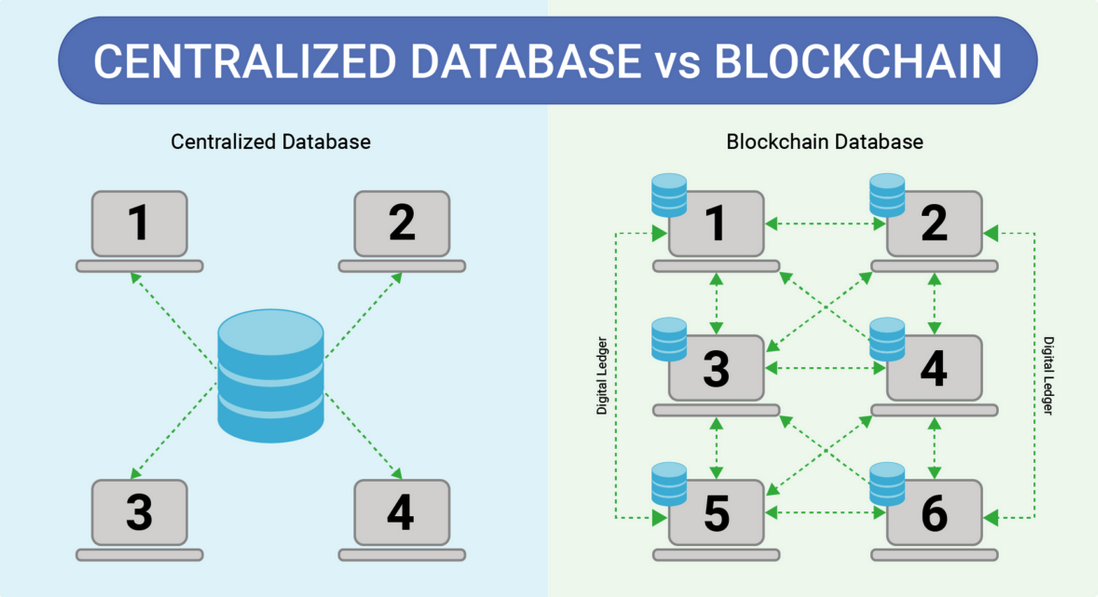
\includegraphics[width=0.8\textwidth]{assets/blockchain-vs-database.png}
    \caption{Centralized vs Blockchain Systems~\cite{blockchainDB}.}
\end{figure}

The use of blockchain technology ensures that certificates are immutable, transparent and accessible to all stakeholders~\cite{alammary2019blockchain}. Moreover, this technology enables the instant verification through cryptographic methods,
eliminating the need for a central authority to manage the registry, thereby reducing the risk of fraud and manipulation.

In contrast to the traditional centralized data-based system, in our opinion, blockchain emerges with a huge influence capable of revolutionizing academic certificate registry systems.
The decision to use blockchain technology as the foundation of our solution is based on the fact that blockchain technology is a key enabler of the \textit{Web3} vision~\cite{buldas2022towards},
which aims to create decentralized and fully distributed applications (\textit{dApps}) that are secure, transparent and trust less where users have full control over their data and digital assets without having a \textbf{single point of failure}.
For the implementation of a blockchain-based solution for our problem it is crucial to understand the foundational concepts that make this technology both revolutionary and reliable.
Central to blockchain's efficacy is the principle of \textit{distributed consensus}~\cite{xiao2020survey}, which ensures the integrity, security and transparency of the ledger like mentioned before.

% Should we add a subsection here where walk deeper into the blockchain technology and its concepts?

Blockchain technology started to gain popularity in 2008 initially described by Satoshi Nakamoto in a white paper entitled `Bitcoin: A Peer-to-Peer Electronic Cash System'~\cite{nakamoto2008bitcoin}.
Although the term blockchain gained popularity in that year, with the introduction of Bitcoin cryptocurrency by Nakamoto, its underlying concepts have been used since the 1980s.
Later in 2004, Harold Thomas Finney II introduced the Reusable Proof of Work (\textit{RPOW}) system~\cite{RPOW}. The RPOW system was a digital
currency system that used a \textit{proof-of-work} that limit the amount of work done by the server and to limit the amount of work done by the client.
The RPOW system was the first system to use a blockchain-like structure to store and verify transactions. Later, in 2009 the first bitcoin transaction was made by Nakamoto
to his friend Hal Finney~\cite{peterson2014hal} where was transferred 10 BTC (bitcoin). This marked the beginning of the blockchain technology era.
In 2013, Vitalik Buterin proposed the concept of \textit{smart contracts} in his white paper `Ethereum: The Ultimate Smart Contract and Decentralized Application Platform'~\cite{buterin2013ethereum}. Upon this publication,
\textit{Ethereum} has launched his own blockchain in 2015.~\cite{reiff2020bitcoin}.

Blockchain can be defined as a time-ordered set of blocks or nodes where each block is cryptographically linked to the previous one forming a chain. All blocks are stored in a decentralized and distributed ledger and become
trustworthy digital records what are not modifiable in practice but very easy to verify. Like mentioned before, there is no centralized or hierarchical structure in the blockchain network and the information is shared by a network of \textit{peers}.

\begin{figure}[h]\label{fig:blockchain}
    \begin{center}
        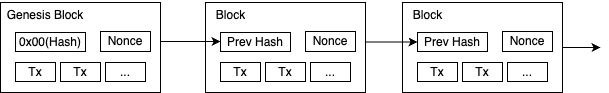
\includegraphics[width=0.8\textwidth]{assets/blockchain.png}
        \caption{Blockchain structure adapted from~\cite{nakamoto2008bitcoin}}
    \end{center}
\end{figure}

As it can be observed in Figure~\ref{fig:blockchain}, each block contains a reliable register of one or more actually executed transactions that are created and exchanged by the network participants (peers) which eventually must modify
its state. To add new information to the chain, a \textbf{consensus} about its truthfulness must be reached among the peers in the network.
For a detailed explanation of consensus mechanism, please refer to Section \ref{subsec:distributed-consensus-mechanisms}.

The content of each transaction that is stored in a single block depends on the specific type of blockchain and its purpose. In our case and very succinctly, the transaction has an `item' that contains information about the academic certificate; we will discuss this in more detail in the next chapters. Other example used nowadays is the Bitcoin, where the main information registered in transactions are exchanges of bitcoins between accounts.

Other important aspect of a chain node and the major reason for its security is the \textbf{hash} function.
This function is used like a digital fingerprint to verify whether or not the data contained in the block has been tampered with. It is created when a new block is added or updated onto the chain.
In the blockchain, each block's hash includes the hash of the previous block, linking them together in a chain. If someone tries to change any information in a block, even just a tiny bit, the hash of that block will change completely. This change would break the link to the next block, making it obvious that the information has been tampered with.
This is the reason why the blockchain is considered tamper-proof and secure.

Some blockchains support the use of \textit{Smart Contracts}~\cite{kaur2023introduction} which are self-executing contracts with the terms of the agreement directly written into code.
These Smart Contracts are a critical component of several applications and platforms using a distributed ledger technology that we will be using in our solution and for better understanding we will explain with
more detail in the next sections.

There are three main types of blockchain~\cite{paul2021blockchain}:

\begin{itemize}
    \item {Public}: is called public if each participants can read and use it to carry out transactions but also
          if everyone can participate in the process of creating the \textbf{consensus} which can be \textit{Proof-of-Work} or \textit{Proof-of-Stake}~\cite{whatIsConsensusCrypto, whatIsConsensus}.
          In this type of blockchain there is no central authority nor a trusted third party to control the network.
          Examples of this type of blockchain are \textbf{Bitcoin}~\cite{nakamoto2008bitcoin} and \textbf{Ethereum}~\cite{tual2015ethereum}. The main advantages of this type of blockchain are:
          \begin{itemize}
              \item High security and privacy,
              \item Open and Flexible Environment,
              \item No regulations,
              \item Full Transparency and Systems,
              \item Distributed, etc.
          \end{itemize}

    \item {Private}: these are restricted and not open, such kind of blockchain also has features of access. This type of blockchains works mostly on closed systems and networks and are usually
          useful in organizations and companies which only selected members can join and access the data. Private blockchains have running only authorized nodes and that means that no one from the outside
          of the private network is able to access the information and data exchanged between two nodes. In this type there is no mining, no proof of work, and no remuneration~\cite{guegan:halshs-01524440}.
          Examples of this type of blockchain are \textbf{Hyperledger Fabric}~\cite{hyperLedger} and \textbf{R3 Corda}~\cite{r3Corda}.
          The main advantages of this type of blockchain are:
          \begin{itemize}
              \item Full of privacy,
              \item High Efficiency,
              \item Faster Transaction,
              \item Better Scalability.
          \end{itemize}
    \item {Consortium~\cite{KASI20221}}: a combination of both public and private blockchains. As in a private blockchain, participants may join the network only by invitation and must be approved by the network owner, however,
          there is not a single organization that has control over the network. Instead, the control is distributed among a group of participants.
          \begin{itemize}
              \item High Security,
              \item High Scalability,
              \item High Efficiency,
              \item High Privacy,
              \item High Flexibility.
          \end{itemize}

\end{itemize}

\subsection*{Distributed Consensus Mechanisms}\label{subsec:distributed-consensus-mechanisms}
\paragraph{}

As mentioned in the beginning of the Section~\ref{sec:blockchain}, the blockchain technology is based on the concept of distributed consensus, which is a procedure used to achieve an
agreement among all the peers of the blockchain network about the present state of the ledger. Through this mechanism, consensus algorithms ensure that all nodes in the network agree on the validity of the transactions and the order in which they are added to the blockchain.
To do a parallelism with the real world, the consensus mechanism is the way that humans agree on the rules of a game, for example, in Monopoly where there are a lot of different ways to win, buying all the properties or end up with a lot of money in the bank
and bankrupt all the other players but no matter what the rules are, everyone has agreed that it is a fair way to end the game~\cite{whatIsConsensus}.
Consensus mechanisms are essential to the security and integrity of the blockchain network, as they prevent malicious actors from altering the ledger and ensure that all transactions are valid and consistent across all nodes.
It prevent the \textit{double-spending} problem, where a user spends the same digital currency more than once, which is a common issue in digital currency systems.

\begin{itemize}
    \item \textbf{Proof-of-Work (PoW)}: this consensus mechanism is the first algorithm used in blockchain technology, introduced by Nakamoto in the Bitcoin white paper~\cite{nakamoto2008bitcoin}.
          In this mechanism, the nodes in the network that engages in mining are known as miners; they compete to solve complex mathematical problems, known as cryptographic puzzles, to validate transactions and add new blocks to the blockchain. These puzzles require miners to find a specific hash value that meets certain criteria, a process that involves extensive computational effort. The first miner to solve the problem is rewarded with a certain amount of cryptocurrency.
          PoW is known for its high energy consumption and slow transaction speeds, as miners must perform a large number of computations to solve the puzzle. However, it is also highly secure and resistant to attacks, as it would require a majority of the network's computing power to alter the blockchain.
          Examples of blockchains that use PoW are Bitcoin and Litecoin~\cite{takashima2018litecoin}.
    \item \textbf{Proof-of-Stake (PoS)}: this mechanism is an algorithm to PoW that aims to reduce energy consumption and increase transaction speeds.
          In PoS, validators are chosen to create new blocks based on the number of coins they hold, rather than the amount of computational power they contribute.
          Unlike PoW, PoS contributors (validators) are not rewarded with new coins, but with transaction fees. PoS is considered more energy-efficient than PoW, and more secure
          against 51\% attacks, as it would require a majority of the network's coins to alter the blockchain. However, as the system is based on the number of coins held by the validators, it can lead to centralization, as those with more coins have more influence over the network.
\end{itemize}

After approaching all three concepts—centralized, distributed, and blockchain systems—we created a summary and made a comparison table (Table~\ref{tab:centralized-vs-distributed-vs-blockchain}) to evaluate their suitability for an academic certificate registry system. From the results in the table, we can conclude that blockchain technology is the most suitable solution. This is due to its decentralized, secure, and tamper-proof nature, which ensures the integrity and authenticity of academic certificates while also providing instant verification and transparency to all stakeholders.

\begin{table}[h]\label{tab:centralized-vs-distributed-vs-blockchain}
    \centering
    \renewcommand{\arraystretch}{1.5} % Default value: 1
    \begin{tabular}{|l|l|l|l|}
        \hline
                     & \textbf{Centralized Systems} & \textbf{Distributed Systems} & \textbf{Blockchain} \\ \hline
        Data Control & Centralized                  & Distributed                  & Fully Distributed   \\ \hline
        Data Storage & Single                       & Multiple                     & Multiple            \\ \hline
        Security     & Low                          & Medium                       & High                \\ \hline
        Privacy      & Low                          & Medium                       & High                \\ \hline
        Trustless    & No                           & No                           & Yes                 \\ \hline
        Scalability  & Low                          & Medium                       & High                \\ \hline
    \end{tabular}
    \caption{Centralized vs Distributed vs Fully Distributed Storage Systems}
\end{table}

\section{Smart Contracts}\label{sec:smart-contracts}
\paragraph{}

Smart Contracts~\cite{vigliotti2021we} are a term that was first introduced by Nick Szabo in 1994~\cite{szabo2017winning} and are self-executing digital agreements that enable two or more parties to exchange
assets or information without the need for a trusted third party.
In the context of our solution, Smart Contracts are the modern version of the traditional paper-based legal agreement, where the terms and conditions of the agreement are written in code and automatically executed when certain conditions are met.
It is an evolving technology that are changing the way that legal agreements are bind to the parties involved in that agreement~\cite{Kaur2023}.

Smart Contracts are computer programmed by a software developer who writes the terms and conditions of the agreement. Despite the automatization of the execution and the certainty that all the parts
involved immediately know the outcome of the agreement, there is no involvement of an intermediary in the process.

However, not all the blockchains support the use of Smart Contracts and there are some challenges that need to be addressed when using this technology.
One of the main challenges due to the blockhains' immutable property, is the impossibility to change or add any term into a contract that is already deployed in the blockchain.
This means that if there is a bug in the code or if there is a need to change the terms of the contract, it is necessary to deploy a new contract with the new terms and conditions.

Saying that, the use of Smart Contracts in our solution is crucial to ensure that the academic certificates are stored and verified by the participants that meets the requirements of the contract.
This will ensure that the certificates are stored in a secure and tamper-proof manner, and that the verification process is transparent and efficient.

\section{Blockchain for Document Registry}\label{sec:blockchain-academic-certificate-registry}
\paragraph{}

As described in Section~\ref{sec:blockchain}, by leveraging the blockchain's decentralization, certificates can be stored across a distributed network,
reducing the risks associated with centralized storage systems such data breaches and corruption.
The immutability of the blockchain brings some advantages and disadvantages to the academic certificate registry system~\cite{nzuva2019smart}.
It is considered as main advantage the fact that certificates are tamper-proof and secure, as they cannot be altered or deleted once they are added to the blockchain. This ensures the
integrity and authenticity of the certificates, making them highly resistant to fraud and manipulation.
However, the immutability of the blockchain brings some challenges to the system. It is impossible to change or delete the certificates once they are added to the blockchain, which will
require a new certificate to be issued in case of any errors or changes in the certificate.

Since we're using Ethereum blockchain, the certificates will be stored onto the chain as a transaction that was deployed by a contract.
This Smart Contract will be responsible for storing and verifying the certificates and will be executed by the participants that meets the requirements of the contract.

\subsection*{Blockchain in Different Sectors}\label{subsec:blockchain-different-sectors}
\paragraph{}

Such implementation is being previously introduced by some institutions and companies. For example, the Massachusetts Institute of Technology (MIT) has developed a blockchain-based system called Blockcerts~\cite{blockcerts}
that allows students to store and share their academic certificates. Additionally, there are some articles that propose the use of blockchain technology for document registry~\cite{app112411811, app14020706}.
In Portugal, institutions from other sectors are also starting to use blockchain technology for registry. For example, a group of people working for Blockchain Portugal~\cite{blockchainPortugal}, in agriculture sector,
have developed a blockchain-based system for making the registry of cherry boxes that are being distributed to the market~\cite{tertuliaCereja}.
This system registers every stop location of each box, from the moment they leave the farm where they were harvested until they are sold to the market. With this, the system makes possible the tracking of the boxes without the need of a centralized authority to manage the registry.
These are good examples of how blockchain technology can be used in different sectors and how it can be used to make the registry of documents or assets in a secure and tamper-proof way keeping the integrity and transparency of the data.